\documentclass{article}
\usepackage{amsmath,amssymb,amsthm,kotex,mdframed,paralist}

\newcounter{num}
%\newcommand{\defi}[1]
%{\bigskip\noindent\refstepcounter{num}\textbf{정의 \arabic{num}) #1}\par}
%\newcommand{\theo}[1]
%{\bigskip\noindent\refstepcounter{num}\textbf{정리 \arabic{num}) #1}\par}
\newcommand{\exam}[1]
{\bigskip\noindent\refstepcounter{num}\textbf{예제 \arabic{num}) #1}\par}
\newcommand{\prob}[1]
{\bigskip\noindent\refstepcounter{num}\textbf{문제 \arabic{num}) #1}\par}
\newcommand{\summ}[1]
{\bigskip\noindent\refstepcounter{num}\textbf{요약 \arabic{num}) #1}\par}

\renewcommand{\figurename}{그림}
%\renewcommand{\proofname}{증명)}
\newcommand{\sol}{\par\bigskip\noindent{\bfseries풀이)}\par}
\newcommand{\ans}[1]{{\raggedleft\textbf{답 : }#1\par}}

\addtolength{\oddsidemargin}{-.875in}
	\addtolength{\evensidemargin}{-.875in}
	\addtolength{\textwidth}{1.75in}

	\addtolength{\topmargin}{-.875in}
	\addtolength{\textheight}{1.75in}
%%%
\begin{document}

\title{혜령 : 01 복습(1)}
\author{}
\date{\today}
\maketitle
\tableofcontents
\newpage

%%
\section{좌표평면과 점}
%
\summ{}
\begin{enumerate}
\item
아래 그림과 같이 왼쪽에서 오른쪽으로 뻗은 반직선을 \(x\)축, 아래에서 위로 뻗은 반직선을 \(y\)축이라고 한다.
\item
\(x\)축과 \(y\)축의 교점을 원점이라고 하고, \(O(0,0)\)으로 표시한다.
\item
\(x\)축과 \(y\)축, 원점을 포함한 2차원 평면을 `좌표평면'이라고 부른다.
\end{enumerate}
\begin{figure}[h!]
\centering
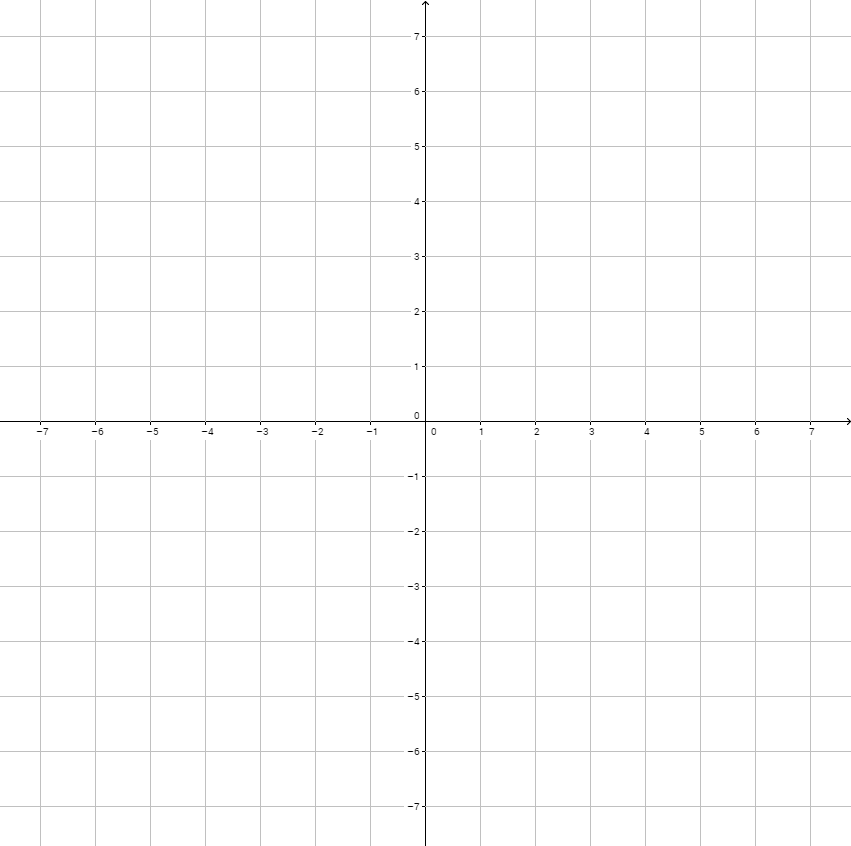
\includegraphics[width=0.5\textwidth]{the_coordinate_plane}
\end{figure}

%
\exam{}
아래 그림에서 \(A=(1,2)\), \(B=(-3,2)\)이다.
\begin{figure}[h!]
\centering
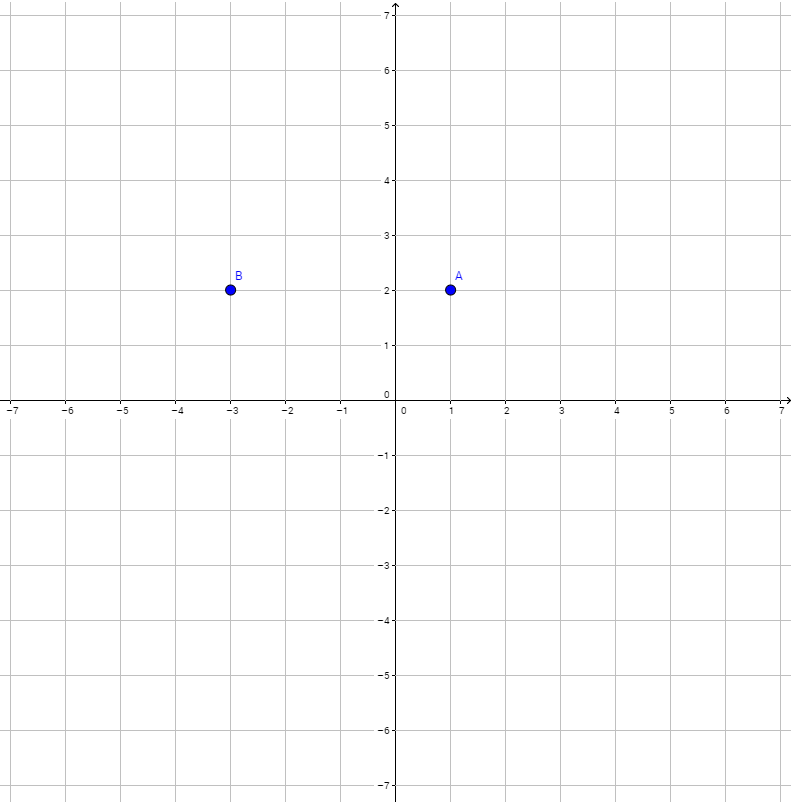
\includegraphics[width=0.5\textwidth]{AB}
\end{figure}

%
\prob{점의 평행이동과 대칭이동}
아래 그림을 보고 다음 물음에 답하시오.
\begin{figure}[h!]
\centering
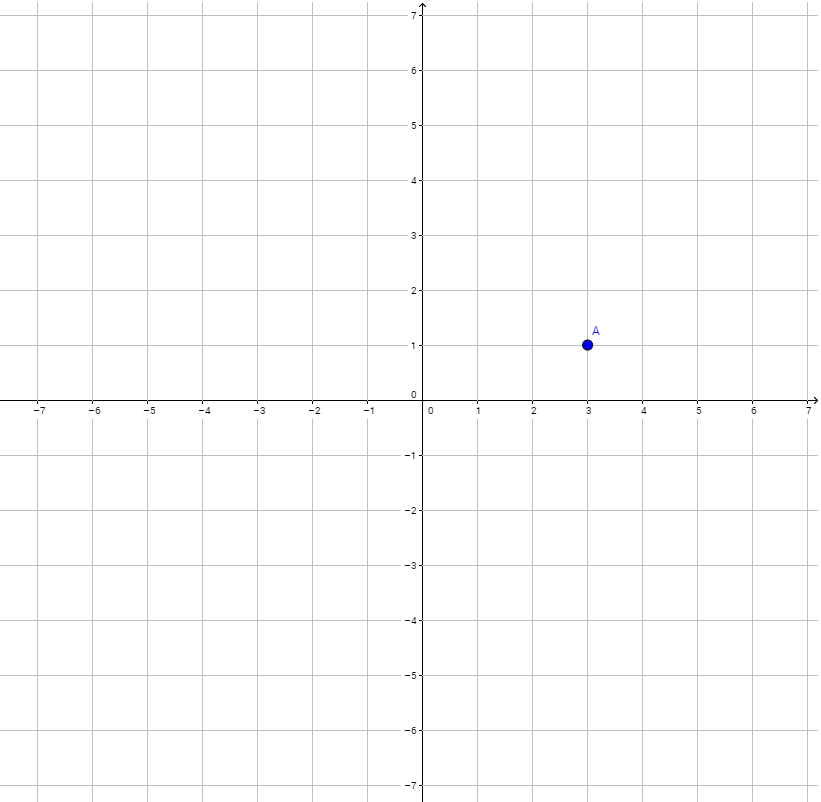
\includegraphics[width=0.5\textwidth]{transfer_and_reflect_a_point_1}
\end{figure}
\begin{enumerate}
\item
\(A\)점의 좌표를 구하시오
\item
\(A\)를 \(x\)축의 방향으로 1만큼, \(y\)축의 방향으로 2만큼 평행이동 시킨 점을 \(A_1\)이라고 할 때, \(A_1\)의 좌표를 구하고 좌표평면 위에 나타내시오.
\item
\(A\)를 \(x\)축을 기준으로 대칭이동 시킨 점을 \(A_2\), \(y\)축을 기준으로 대칭이동 시킨 점을 \(A_3\), 원점을 기준으로 대칭이동 시킨 점을 \(A_4\)라고 할 때, \(A_2\), \(A_3\), \(A_4\)의 좌표를 구하고 좌표평면 위에 나타내시오.
\end{enumerate}

\newpage
%
\prob{점의 평행이동과 대칭이동(2)}
\(B=(-2,3)\)일 때 다음 물음에 답하시오.
\begin{figure}[h!]
\centering
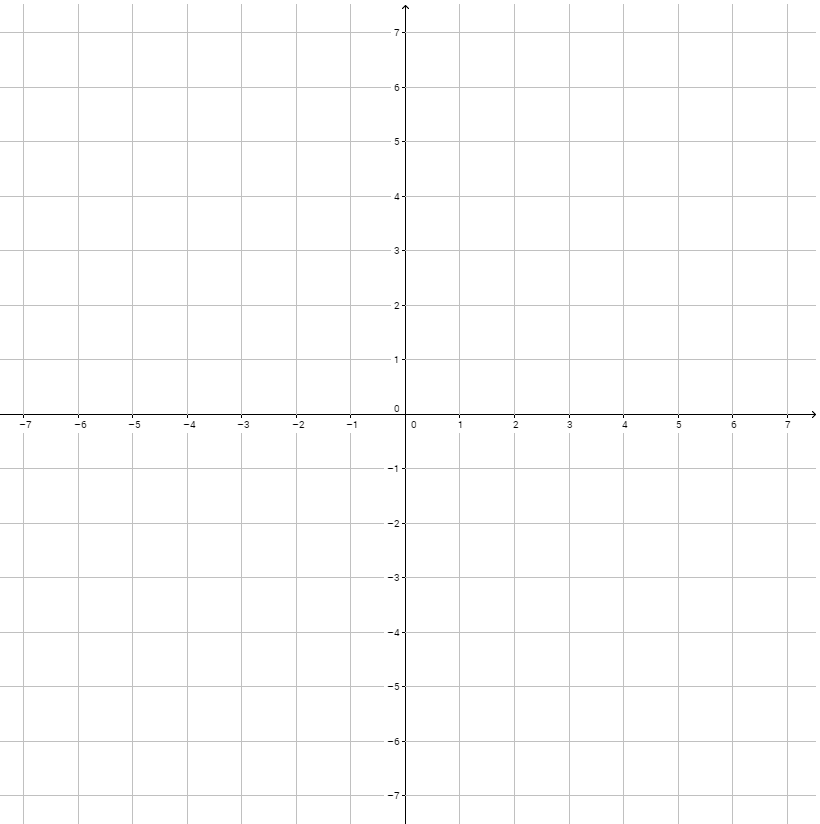
\includegraphics[width=0.5\textwidth]{transfer_and_reflect_a_point_2}
\end{figure}
\begin{enumerate}
\item
\(B\)점을 좌표평면 내에 표시하시오.
\item
\(B\)를 \(x\)축의 방향으로 3만큼, \(y\)축의 방향으로 -2만큼 평행이동 시킨 점을 \(B_1\)이라고 할 때, \(B_1\)의 좌표를 구하고 좌표평면 위에 나타내시오.
\item
\(B\)를 \(x\)축을 기준으로 대칭이동 시킨 점을 \(B_2\), \(y\)축을 기준으로 대칭이동 시킨 점을 \(B_3\), 원점을 기준으로 대칭이동 시킨 점을 \(B_4\)라고 할 때, \(B_2\), \(B_3\), \(B_4\)의 좌표를 구하고 좌표평면 위에 나타내시오.
\end{enumerate}

%%
\section{직선}
%
\exam{}
식 \(y=x+3\)의 그래프를 그려보자.
즉 \(y=x+3\)를 만족하는 모든 \((x,y)\)를 좌표 평면 내에 표시해보자.
\begin{itemize}
\item
만약 \(x=0\)이면 \(y=3\)이어야 한다.
그러므로 \((0,3)\)를 표시하자.
\item
만약 \(x=1\)이면 \(y=4\)이어야 한다.
그러므로 \((1,4)\)를 표시하자.
\item
만약 \(x=2\)이면 \(y=5\)이어야 한다.
그러므로 \((2,5)\)를 표시하자.
\item
만약 \(x=3\)이면 \(y=6\)이어야 한다.
그러므로 \((3,6)\)를 표시하자.
\item
만약 \(x=-1\)이면 \(y=2\)이어야 한다.
그러므로 \((-1,2)\)를 표시하자.
\item
만약 \(x=-2\)이면 \(y=1\)이어야 한다.
그러므로 \((-2,1)\)를 표시하자.
\item
만약 \(x=0.5\)이면 \(y=3.5\)이어야 한다.
그러므로 \((0.5,3.5)\)를 표시하자.
\end{itemize}
이 일곱 개의 점들을 모두 좌표 평면 위에 표시하면 아래 그림과 같다.
\newpage
\begin{figure}[h!]
\centering
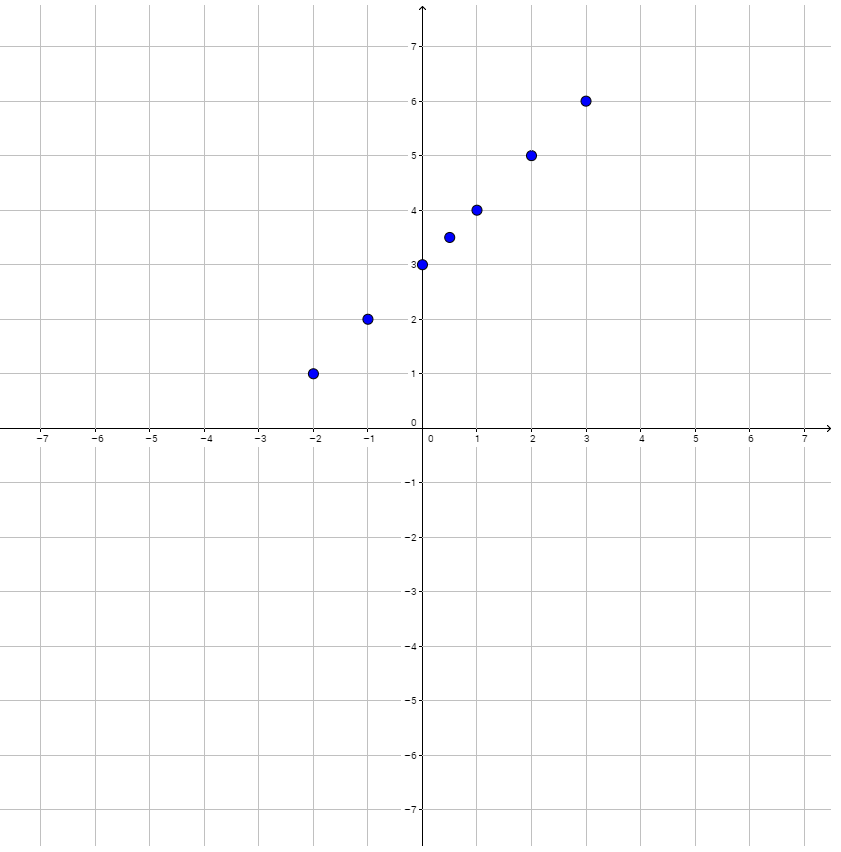
\includegraphics[width=0.5\textwidth]{y=x+3_1}
\end{figure}

따라서 \(y=x+3\)을 만족하는 모든 \((x,y)\)들을 모두 표시하면 한 개의 직선이 만들어진다는 것을 추정할 수 있다.
다음은 \(y=x+3\)의 그래프이다.
\begin{figure}[h!]
\centering
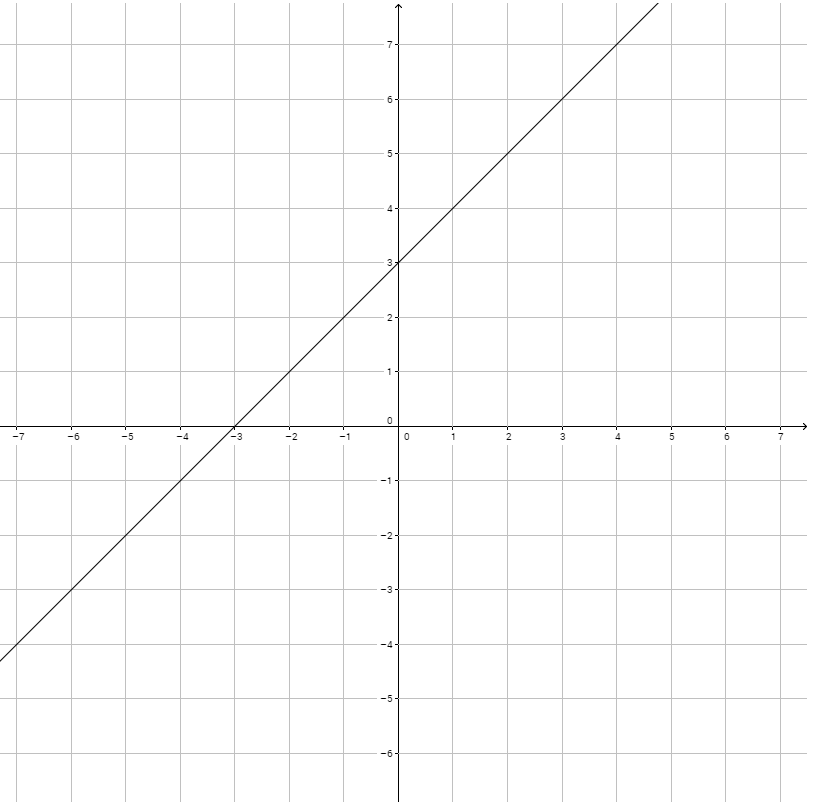
\includegraphics[width=0.5\textwidth]{y=x+3_2}
\end{figure}

%
\prob{}
다음 식의 그래프를 그려라.
\begin{enumerate}
\item
\(y=x\)
\item
\(y=x+1\)
\item
\(y=x-2\)
\item
\(y=x-\frac12\)
\end{enumerate}
\newpage

%
\exam{}
식 \(y=-2x+4\)의 그래프를 그려보자.
즉 \(y=-2x+4\)를 만족하는 모든 \((x,y)\)를 좌표 평면 내에 표시해보자.
\begin{itemize}
\item
만약 \(x=0\)이면 \(y=4\)이어야 한다.
그러므로 \((0,4)\)를 표시하자.
\item
만약 \(x=1\)이면 \(y=2\)이어야 한다.
그러므로 \((1,2)\)를 표시하자.
\item
만약 \(x=2\)이면 \(y=0\)이어야 한다.
그러므로 \((2,0)\)를 표시하자.
\item
만약 \(x=3\)이면 \(y=-2\)이어야 한다.
그러므로 \((3,-2)\)를 표시하자.
\item
만약 \(x=-1\)이면 \(y=6\)이어야 한다.
그러므로 \((-1,6)\)를 표시하자.
\end{itemize}
이번에는 다섯 개의 점들만을 찍었다.
이 다섯 개의 점들을 좌표 평면 위에 나타내면 아래 그림과 같고,
\begin{figure}[h!]
\centering
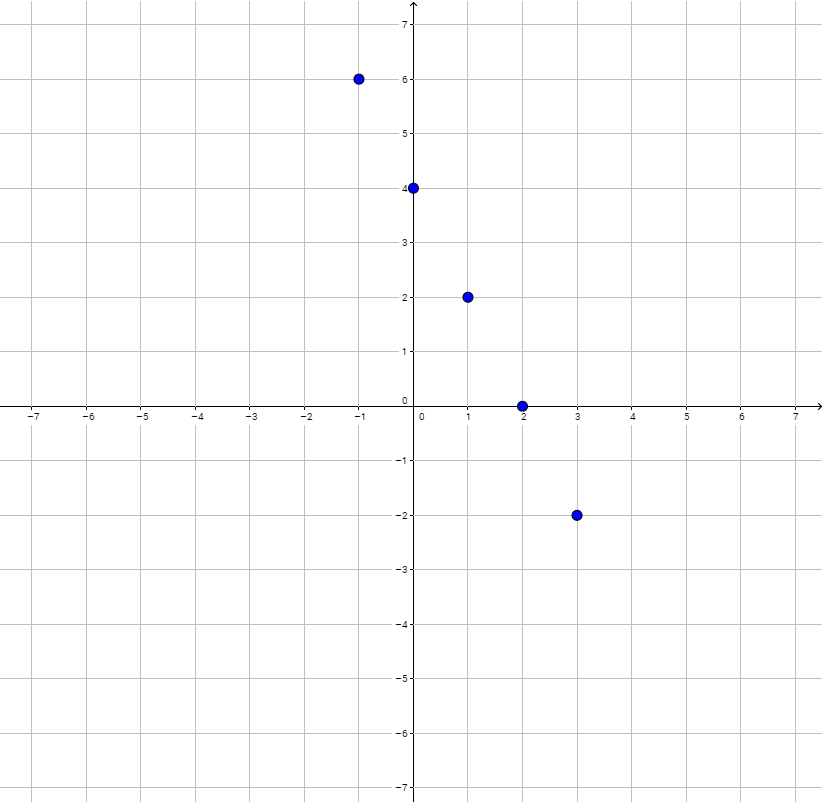
\includegraphics[width=0.5\textwidth]{y=-2x+4_1}
\end{figure}

따라서 \(y=-2x+4\)을 만족하는 모든 \((x,y)\)들을 모두 표시하면 한 개의 직선이 만들어진다는 것을 추정할 수 있다.
다음은 \(y=-2x+4\)의 그래프이다.
\begin{figure}[h!]
\centering
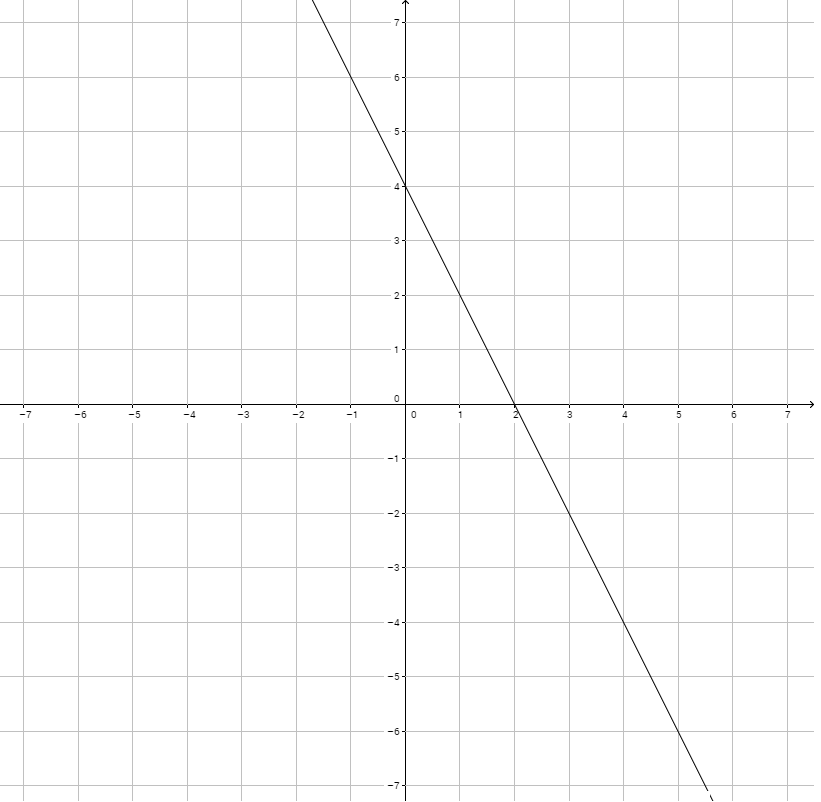
\includegraphics[width=0.5\textwidth]{y=-2x+4_2}
\end{figure}

%
\prob{}
다음 식의 그래프를 그려라.
\begin{enumerate}
\item
\(y=2x\)
\item
\(y=2x-2\)
\item
\(y=3x+1\)
\item
\(y=-x+4\)
\item
\(y=-2x+6\)
\item
\(y=-3x\)
\end{enumerate}

%
\exam{}
식 \(y=\frac12x+1\)의 그래프를 그려보자.
즉 \(y=\frac12x+1\)를 만족하는 모든 \((x,y)\)를 좌표 평면 내에 표시해보자.
\begin{itemize}
\item
만약 \(x=0\)이면 \(y=1\)이어야 한다.
그러므로 \((0,1)\)를 표시하자.
\item
만약 \(x=2\)이면 \(y=2\)이어야 한다.
그러므로 \((2,2)\)를 표시하자.
\item
만약 \(x=4\)이면 \(y=3\)이어야 한다.
그러므로 \((4,3)\)를 표시하자.
\item
만약 \(x=6\)이면 \(y=4\)이어야 한다.
그러므로 \((6,4)\)를 표시하자.
\item
만약 \(x=-2\)이면 \(y=0\)이어야 한다.
그러므로 \((-2,0)\)를 표시하자.
\item
만약 \(x=-4\)이면 \(y=-1\)이어야 한다.
그러므로 \((-4,-1)\)를 표시하자.
\end{itemize}
계산을 편하게 하기 위해 \(y\)값을 정수로 만들려고 일부러 \(x\)에 짝수만을 넣었다.
이 점들을 좌표 평면 위에 나타내면 아래 그림과 같고,
\begin{figure}[h!]
\centering
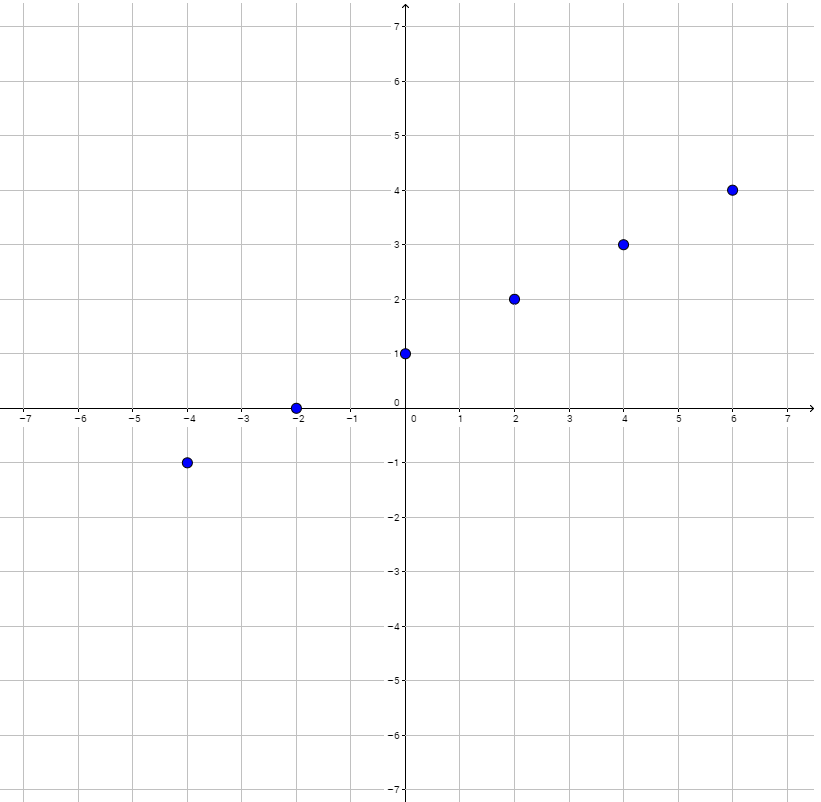
\includegraphics[width=0.5\textwidth]{third_graph_1}
\end{figure}

\newpage
따라서 \(y=\frac12x+1\)을 만족하는 모든 \((x,y)\)들을 모두 표시하면 한 개의 직선이 만들어진다는 것을 추정할 수 있다.
다음은 \(y=\frac12x+1\)의 그래프이다.
\begin{figure}[h!]
\centering
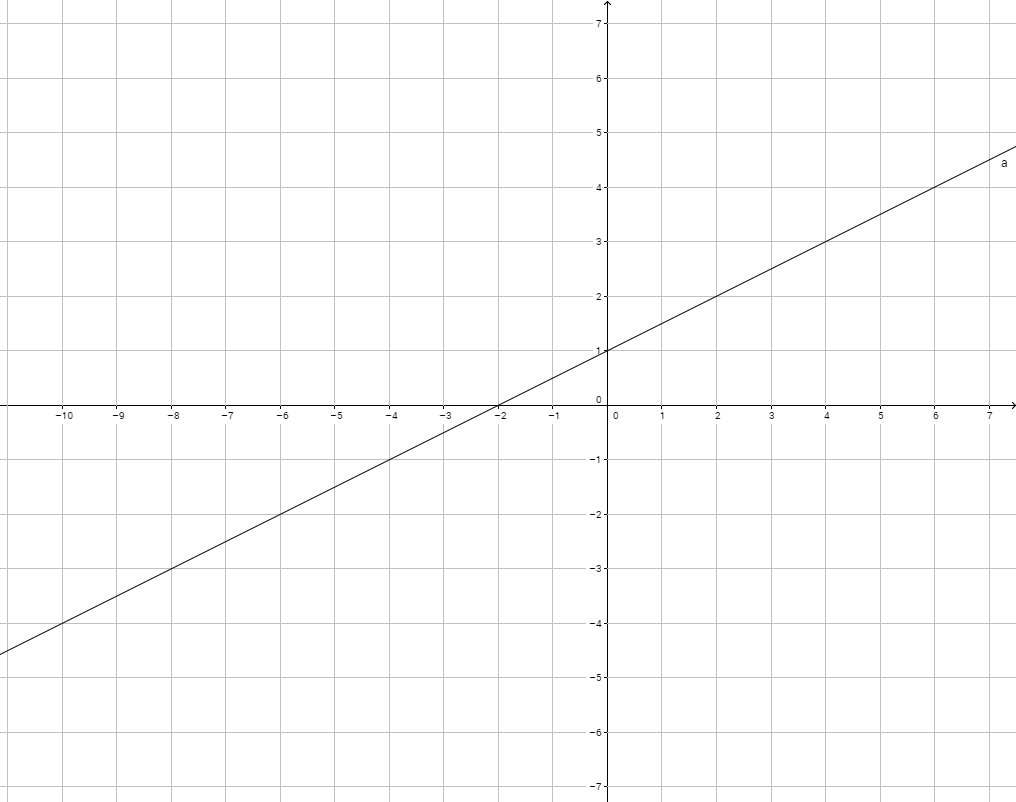
\includegraphics[width=0.5\textwidth]{third_graph_2}
\end{figure}

%
\prob{}
다음 식의 그래프를 그려라.
\begin{enumerate}
\item
\(y=-\frac12x+2\)
\item
\(y=\frac13x-1\)
\item
\(y=\frac32x\)
\end{enumerate}
\newpage

%
\exam{기울기}
세 식
\begin{gather*}
y=x+3\\
y=-2x+4\\
y=\frac12x+1
\end{gather*}
의 그래프를 아래와 같이 한 그림에 그려보았다.
\begin{figure}[h!]
\centering
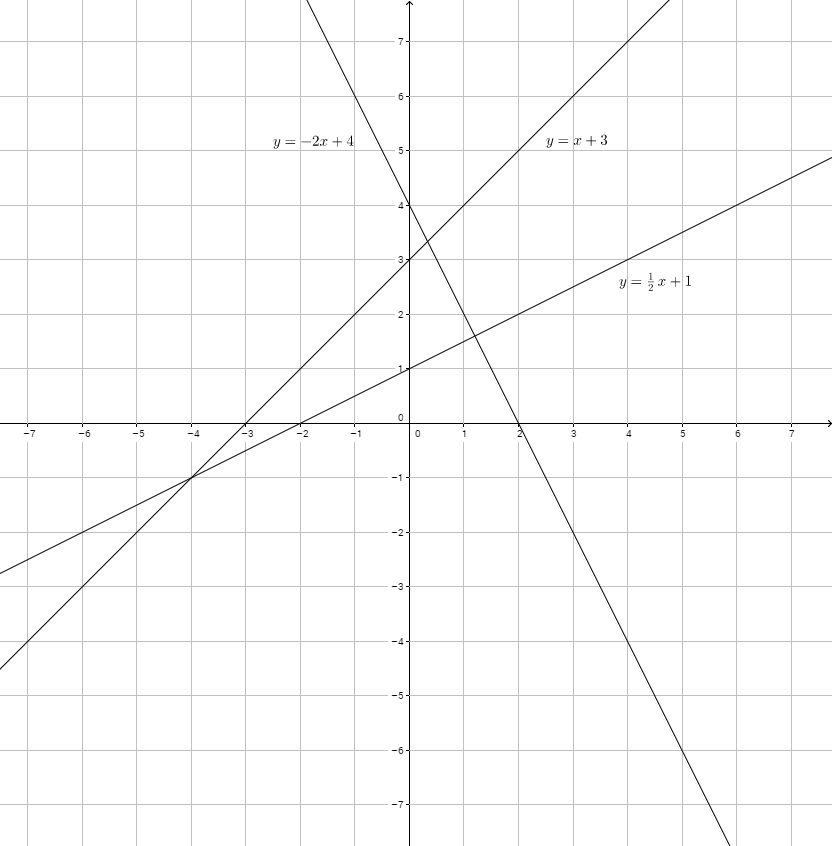
\includegraphics[width=0.5\textwidth]{three_lines}
\end{figure}

\(y=x+3\)의 그래프는 \(x\)축 방향으로 1만큼 증가할 때마다 \(y\)의 값이 1만큼 증가한다.
\(y=-2x+4\)의 그래프는 \(x\)축 방향으로 1만큼 증가할 때마다 \(y\)의 값이 2만큼 감소한다.

이와 같이, 직선에서 \(x\)축 방향으로 1만큼 증가할 때, \(y\)증가 혹은 감소량을 `기울기'라고 부른다.

\(y=\frac12x+1\)의 경우 \(x\)축 방향으로 2만큼 증가할 때마다 \(y\)의 값이 1만큼 증가한다.
따라서 \(x\)축 방향으로 1만큼 증가할 때마다 \(\frac12\)만큼 증가하며, 기울기는 \(\frac12\)이다.
\newpage

%
\exam{}
\begin{figure}[h!]
\centering
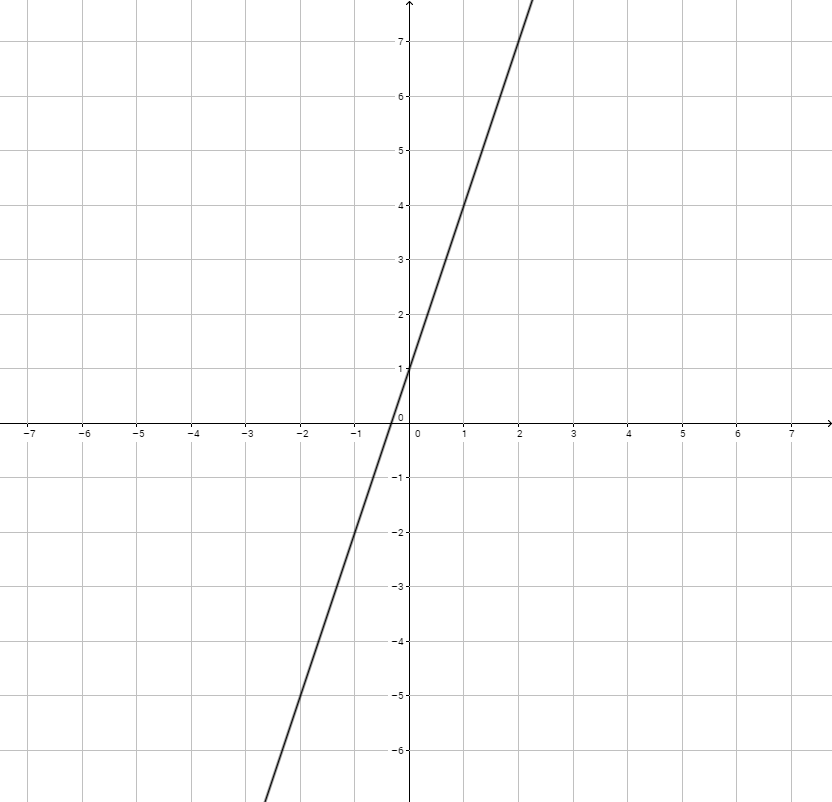
\includegraphics[width=0.45\textwidth]{y=3x+1}
~
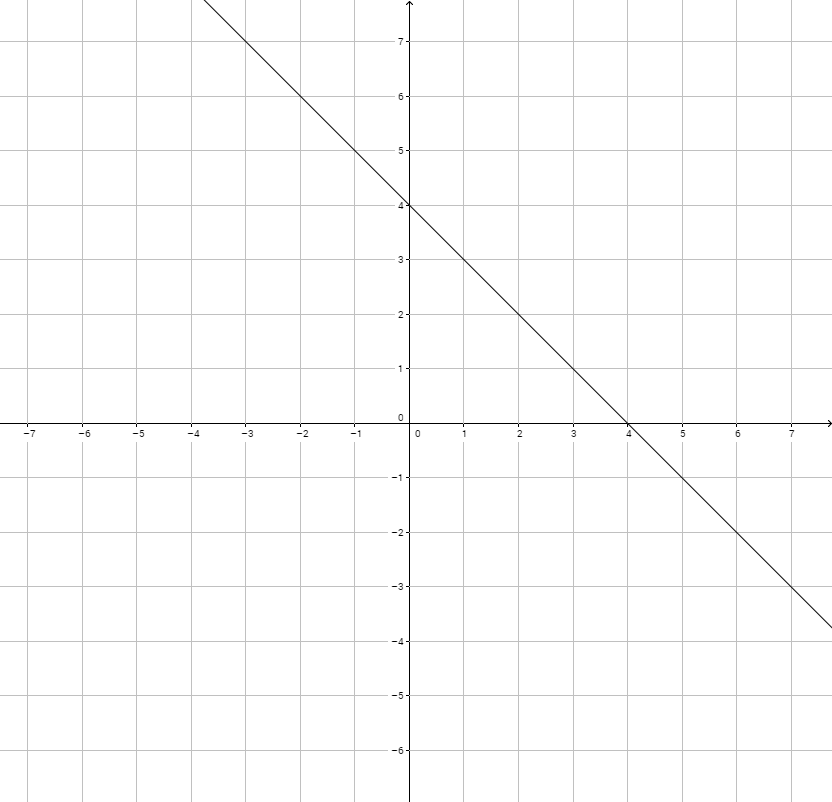
\includegraphics[width=0.45\textwidth]{y=-x+4}\\
(1)\qquad\qquad\qquad\qquad\qquad\qquad\qquad\quad(2)\\
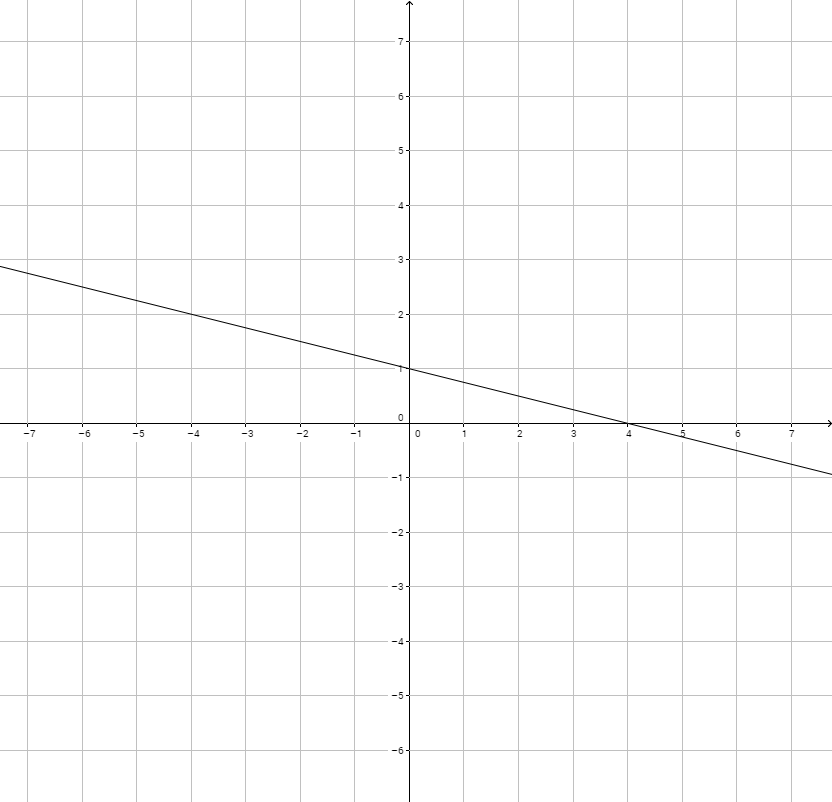
\includegraphics[width=0.45\textwidth]{y=-onefourthx+1}
~
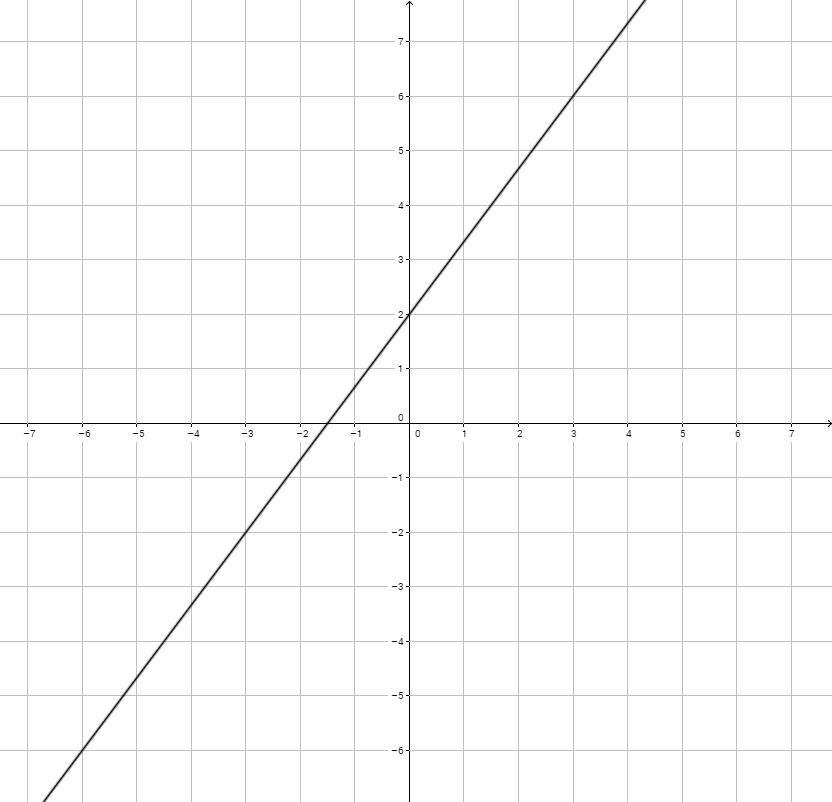
\includegraphics[width=0.45\textwidth]{y=fourthirdx+2}\\
(3)\qquad\qquad\qquad\qquad\qquad\qquad\qquad\quad(4)
\end{figure}
위 그림에서 (1)의 기울기는 3이고, (2)의 기울기는 \(-1\)이다.

(3)에서, \(x\)가 \(0\)에서 \(4\)로 4만큼 증가하면, \(y\)는 \(1\)에서 \(0\)으로 \(-1\)만큼 감소한다.
즉 \(x\)가 \(1\)만큼 증가할 때 \(y\)는 \(\frac14\)만큼 감소한 셈이다.
따라서 기울기는 \(-\frac14\)이다.

(4)에서 \(x\)가 \(0\)에서 \(3\)으로 3만큼 증가하면, \(y\)는 \(2\)에서 \(6\)으로 \(4\)만큼 증가한다.
즉 \(x\)가 \(1\)만큼 증가할 때 \(y\)는 \(\frac43\)만큼 증가한 셈이다.
따라서 기울기는 \(\frac43\)이다.

\newpage
%
\prob{}
\begin{figure}[h!]
\centering
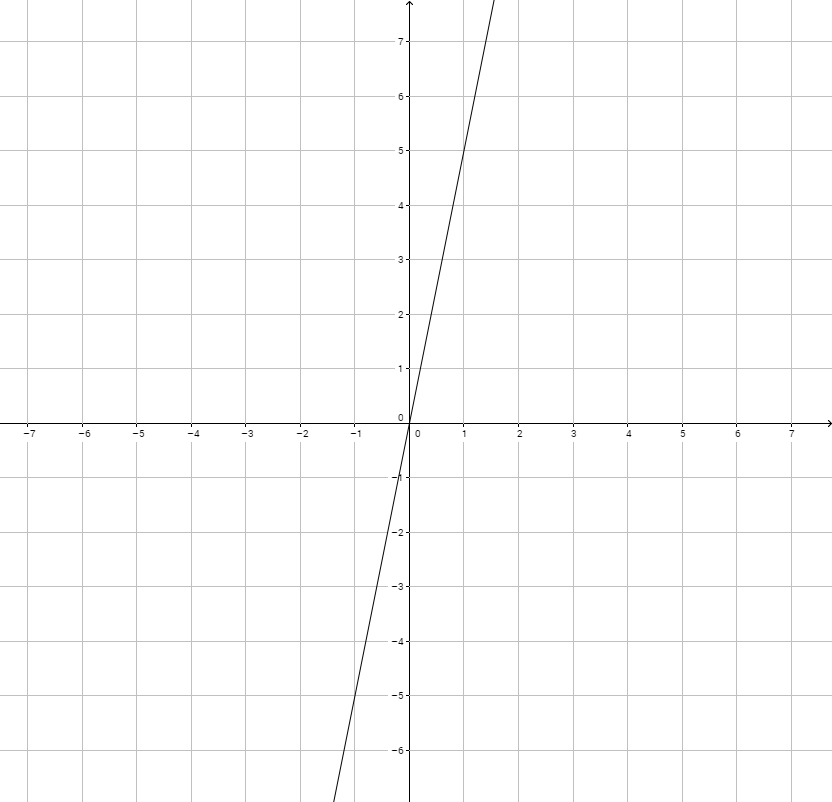
\includegraphics[width=0.45\textwidth]{y=5x}
~
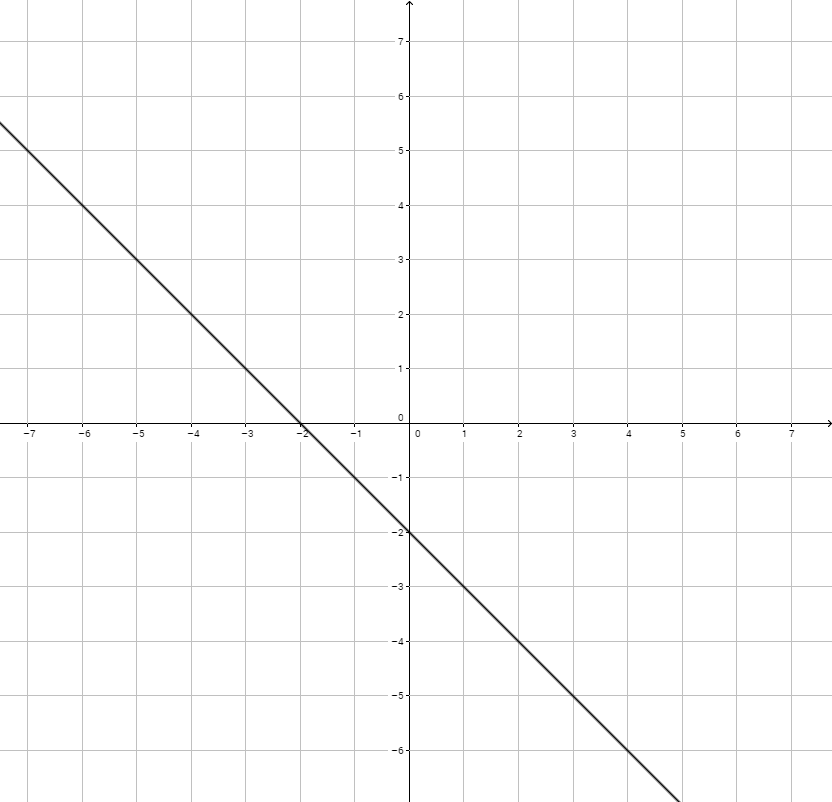
\includegraphics[width=0.45\textwidth]{y=-x-2}\\
(1)\qquad\qquad\qquad\qquad\qquad\qquad\qquad\quad(2)\\
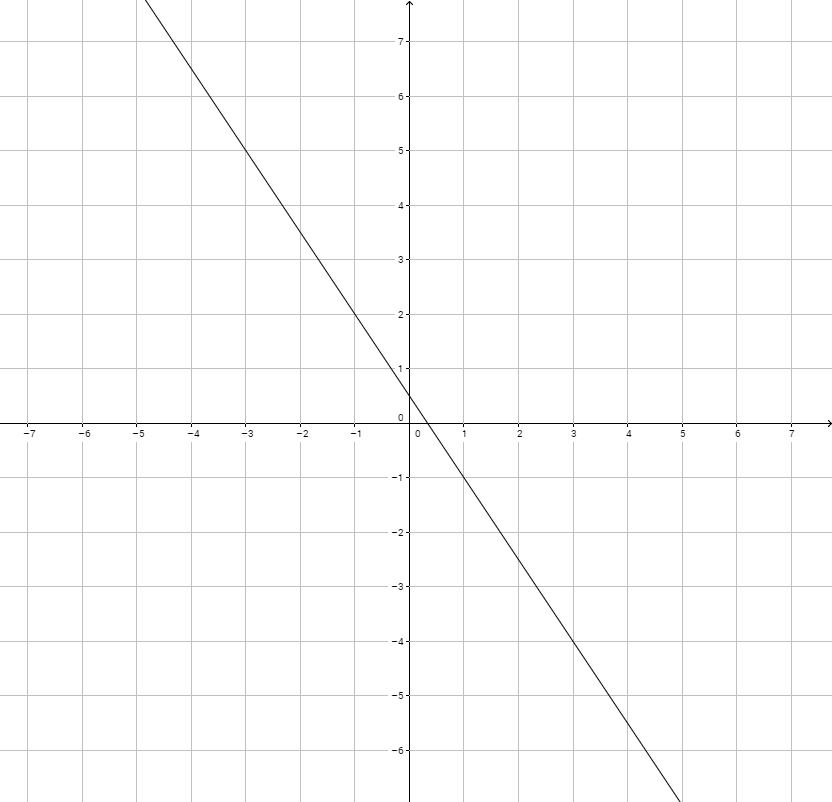
\includegraphics[width=0.45\textwidth]{y=-threehalfx+onehalf}
~
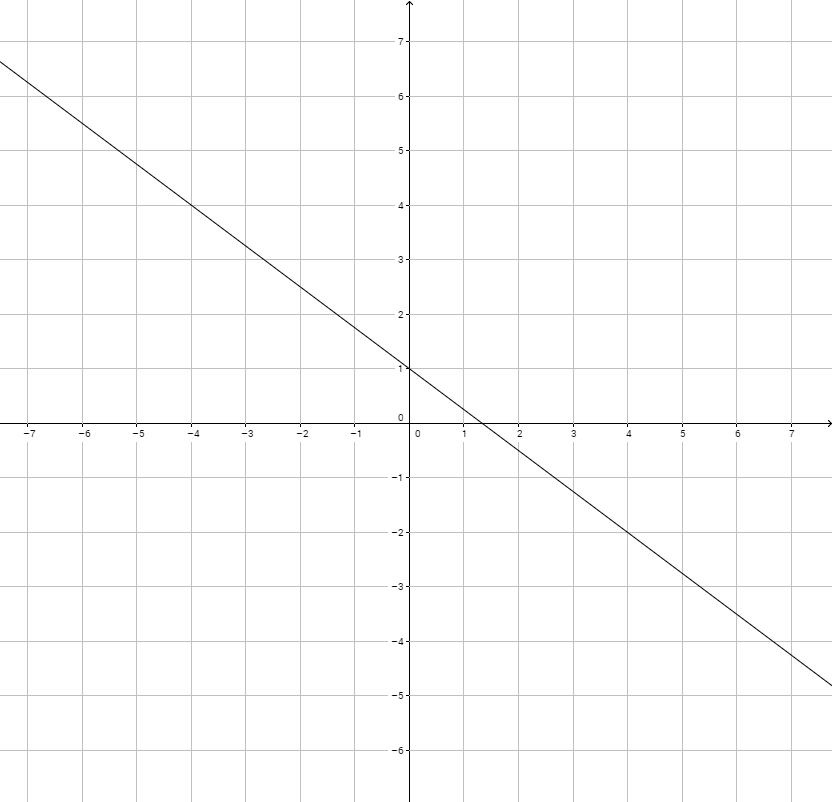
\includegraphics[width=0.45\textwidth]{y=threefourthx+1}\\
(3)\qquad\qquad\qquad\qquad\qquad\qquad\qquad\quad(4)
\end{figure}
다음 직선들의 기울기를 구하시오.

\newpage
%
\summ{}
\begin{enumerate}
\item
그래프와 \(x\)축이 만나는 점의 \(x\)좌표를 \(x\)절편이라고 부른다.
\item
그래프와 \(y\)축이 만나는 점의 \(y\)좌표를 \(y\)절편이라고 부른다.
\item
식 \(y=mx+n\)의 그래프는 기울기가 \(m\)이고, \(y\)절편이 \(n\)인 직선이다.
\item
\(y=mx+n\)와 같은 \(x\)와 \(y\) 사이의 대응관계를 `일차함수'라고 부른다.
\item
함수 \(y=x\)는 특별히 `항등함수'라고 부른다.
\item
\(y=mx+n\)와 같은 식을 `직선의 방정식'이라고 부른다.
\(m\)이 유리수일 경우 이 식을 변형해 \(ax+by+c=0\)꼴로 만들기도 한다.
\end{enumerate}

%
\exam{}
예제 12에서 (1)의 기울기는 3이고 \(y\)절편이 1이므로 직선의 방정식은 \(y=3x+1\)이다.
(2)의 기울기는 \(-1\)이고 \(y\)절편이 \(4\)이므로 직선의 방정식은 \(y=-x+4\)이다.
(3)의 기울기는 \(-\frac14\)이고 \(y\)절편이 \(1\)이므로 직선의 방정식은 \(y=-\frac14x+1\)이다.
(4)의 기울기는 \(\frac43\)이고 \(y\)절편이 \(2\)이므로 직선의 방정식은 \(y=\frac43x+2\)이다.

(3)과 (4)의 경우, 식을 정리해 \(x+4y-4=0\)과 \(4x-3y+6=0\)으로 나타내기도 한다.

%
\prob{}
문제 13에 나타난 직선들의 방정식을 구하시오.

%
\prob{}
다음 직선의 방정식들을 좌표 평면 위에 나타내시오.
\begin{enumerate}
\item
\(y=2x+5\)
\item
\(y=-x-4\)
\item
\(y=\frac12x\)
\item
\(y=-\frac32x+2\)
\item
\(2x+3y-6=0\)
\item
\(3x+4y-20=0\)
\item
\(-3x+y=0\)
\item
\(x+y=2\)
\item
\(x-y=3\)
\item
\(x+2y=4\)
\end{enumerate}

%
\exam{}
식 \(y=0\)를 생각하자.
이 식은 \(y=0\cdot x+0\)이라고 해석될 수 있다.
즉, 기울기가 0이고, \(y\)절편도 0인 직선이므로, \(x\)축이다.
한편 \(y=0\)인 모든 점들 \((x,y)\)을 표시하면, \(x\)축을 이룬다.
어떤 의미로 해석하건, 식 \(y=0\)이 나타내는 직선은 \(x\)축이다.

반대로 \(x=0\)이 나타내는 직선은 \(y\)축이다. 

%
\summ{}
\begin{enumerate}
\item
\(x=a\)가 나타내는 직선은 \((a,0)\)을 지나고 \(y\)축에 평행한 직선이다.
\item
\(y=b\)가 나타내는 직선은 \((0,b)\)을 지나고 \(x\)축에 평행한 직선이다.
\end{enumerate}

%
\summ{}
다음은 각각 \(x=2\), \(y=-3\)을 나타낸 직선이다.

\begin{figure}[h!]
\centering
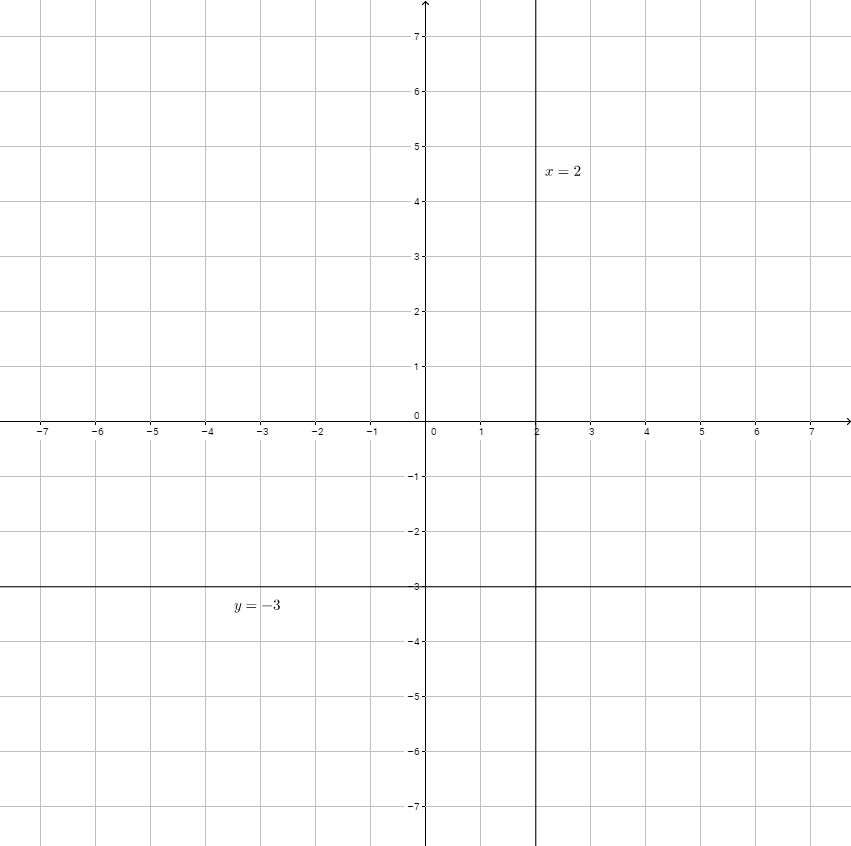
\includegraphics[width=0.5\textwidth]{x=2,y=-3}
\end{figure}

%%
\section{두 직선 사이의 교점}

%
\exam{}
두 직선 \(y=x+3\)과 \(y=-2x+6\) 사이의 교점을 구해보자.
직선 \(y=x+3\)는 \(y=x+3\)를 만족시키는 모든 \((x,y)\)를 의미하고
직선 \(y=-2x+6\)는 \(y=-2x+6\)를 만족시키는 모든 \((x,y)\)를 의미하므로
두 식을 연립하여 두 식을 모두 만족시키는 \((x,y)\)를 찾아냄으로써 교점을 구해낼 수 있다.
\[x+3=y=-2x+6\]
이므로
\[3x=3\]
이고, 따라서
\[x=1\]
이다.
이것을 첫 번째 식에 대입하면(두 번째 식에 대입해도 된다.)
\[y=4\]
를 얻는다.
따라서 구하는 교점은 \((1,4)\)이다.
이것은 두 직선의 방정식을 연립함으로써 얻어진다.
실제 그림을 그려봐도 두 직선의 교점이 \((1,4)\)임을 확인할 수 있다.
\begin{figure}[h!]
\centering
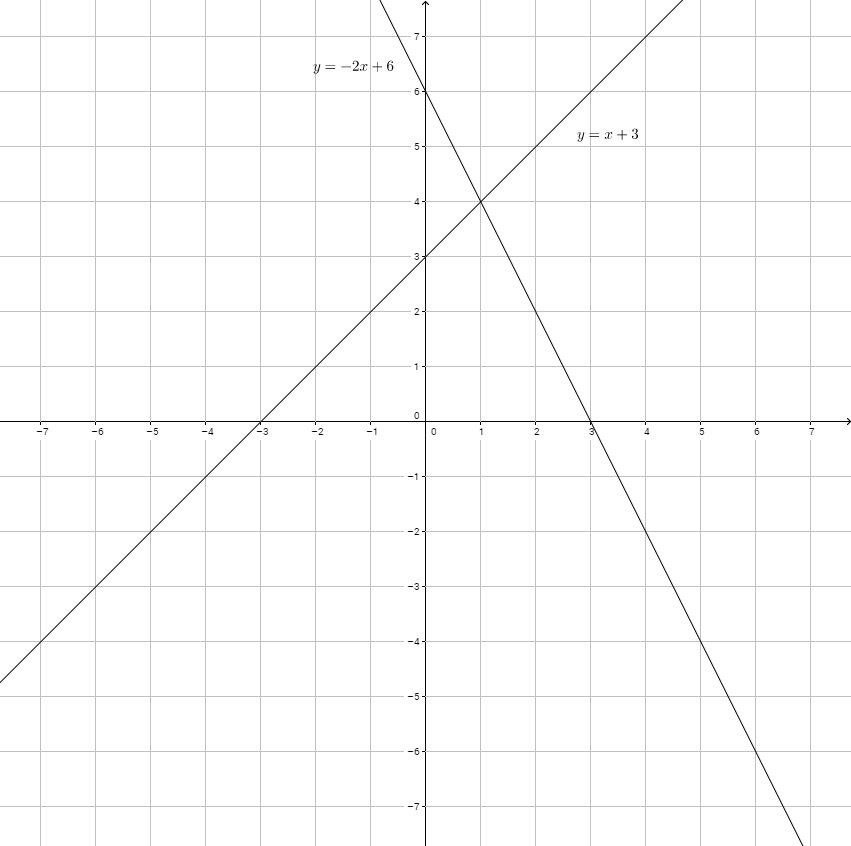
\includegraphics[width=0.5\textwidth]{the_intersect_of_two_lines}
\end{figure}

\newpage
%
\prob{}
다음 두 직선의 교점을 구하시오.
\begin{enumerate}
\item
\(y=2x+1\), \(y=\frac12x+4\)
\item
\(y=x+3\), \(y=3x-1\)
\item
\(y=x-3\), \(x+y=7\)
\item
\(2x+y=5\), \(2x-y=1\)
\item
\(x+2y=-3\), \(3x-y=-2\)
\item
\(x=3\), \(y=3x-4\)
\end{enumerate}

\end{document}